
\chapter{Introduction}\label{victor protocolo hpv redes.doc julio 2016}


%Algo importante que contar
One of the biggest scientific discoveries in the past 30 years was the connection between human papillomavirus infection of the cervix and cervical cancer. This achievement resulted from the original seminal findings by Harald zur Hausen and his group, they found that human papillomavirus genotype 16 can be detected in cervical cancer tissue. 
\begin{figure}[ht]
	\centering
	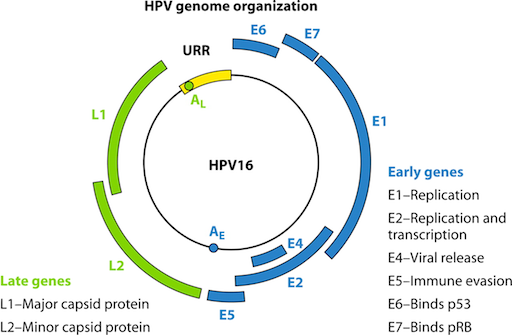
\includegraphics[scale=0.7]{IMG/genoma.png}
	\caption{Cartoon illustrating the genomic organization of a typical mucosal high-risk HPV. The genome contains early and late regions (E), which relate to the positions of the genes within the genome and their timing of expression during the viral life cycle. The early region carries a number of genes which function at the level of viral replication and transcription, i.e., E2, E1, E6, and E7. E2 encodes a protein which has an auxiliary role in viral replication and also functions at the level of transcriptional regulation of the viral early genes. The E6 and E7 genes encode the major transforming proteins of the oncogenic HPVs. The late region (L) encodes viral structural proteins, with L1 being the major capsid protein and L2 being the minor capsid protein.}
	\label{genoma}
\end{figure}
%doi: 10.1128/CMR.05028-11 Clin. Microbiol. Rev. April 2012 vol. 25 no. 2 215-222 1 April 2012

%Foto del HPV-16 con Cryo-EM (nobel química 2017)

The finding was followed by epidemiologists, molecular biologists, vaccinologists, and clinicians culminating in 2006 with the development of effective prophylactic vaccines for human papillomavirus, which have the means to prevent 70-80\% of cervical cancer. Zur Hausen was awarded the Nobel Prize in Physiology or Medicine in 2008, in recognition of his discovery.

\begin{figure}[ht]
	\centering
	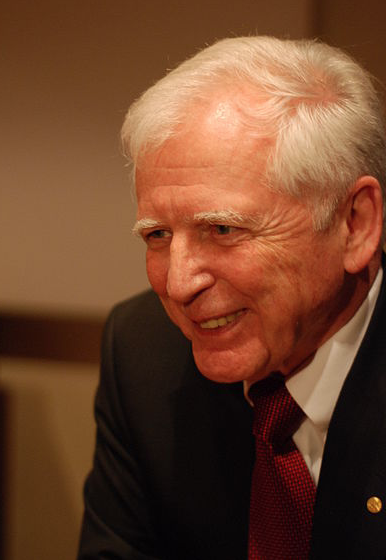
\includegraphics[scale=0.7]{IMG/zurHausen.png}
	\caption{Harald zur Hausen (born 11 March 1936) is a German virologist and professor emeritus. He has done research on cancer of the cervix, where he discovered the role of papilloma viruses, for which he received the Nobel Prize in Physiology or Medicine 2008.}
	\label{zurHausen}
\end{figure} 
%Foto de Zur Hausen

%Datos de lo malo que es
HPV types are often referred to as low risk (LR) wart causing or high risk (HR) cancer causing, based on whether they put a person at risk for cancer.  The types of HPV that can cause genital warts are not the same as the types that can cause cancer.
Persistent human papillomavirus (HPV) infections with genotypes 16 and 18 are responsible for about 70\% of all cervical cancer 
%Clifford GM, Rana RK, Franceschi S, Smith JS, Gough G, Pimenta JM. Human papillomavirus genotype distribution in low-grade cervical lesions: comparison by geographic region and with cervical cancer. Cancer Epidemiol Biomarkers Prev. 2005;14:1157–1164. doi: 10.1158/1055-9965.EPI-04-0812.
%Munoz N, Bosch FX, de Sanjosé S, Herrero R, Castellsague X, Shah KV, et al. Epidemiologic classification of human papillomavirus types associated with cervical cancer. N Engl J Med. 2003;348:518–527. doi: 10.1056/NEJMoa021641.
, with 40-85\% of other anogenital cancers: anal, penile, vaginal, and vulvar cancer, and also 16-28\% of the head and neck cancers.
%%WHO International Agency for Research on Cancer. IARC Monographs on the Evaluation of Carcinogenic Risk to Humans. Human Papillomavirusses. Volume 90. 2007.
%https://www.ncbi.nlm.nih.gov/pmc/articles/PMC4331443/

HPV is a cause of other non malignant diseases, to mention genotypes 6 and 11 cause about 90\% of anogenital warts, and secondarily juvenile onset of recurrent respiratory papillomatosis.
%Lacey CJ, Lowndes CM, Shah KV. Chapter 4: Burden and management of non-cancerous HPV-related conditions: HPV-6/11 disease. Vaccine. 2006;24(Suppl 3):S35–S41. doi: 10.1016/j.vaccine.2006.06.015.

% Literatura dura
Genital human papillomavirus (HPV) is the most common sexually transmitted infection in the United States. More than 40 HPV types can infect the genital areas of men and women, including the skin of the penis, vulva (area outside the vagina), and anus, and the linings of the vagina, cervix, and rectum. These types can also infect the lining of the mouth and throat.

\begin{figure}[ht]
	\centering
	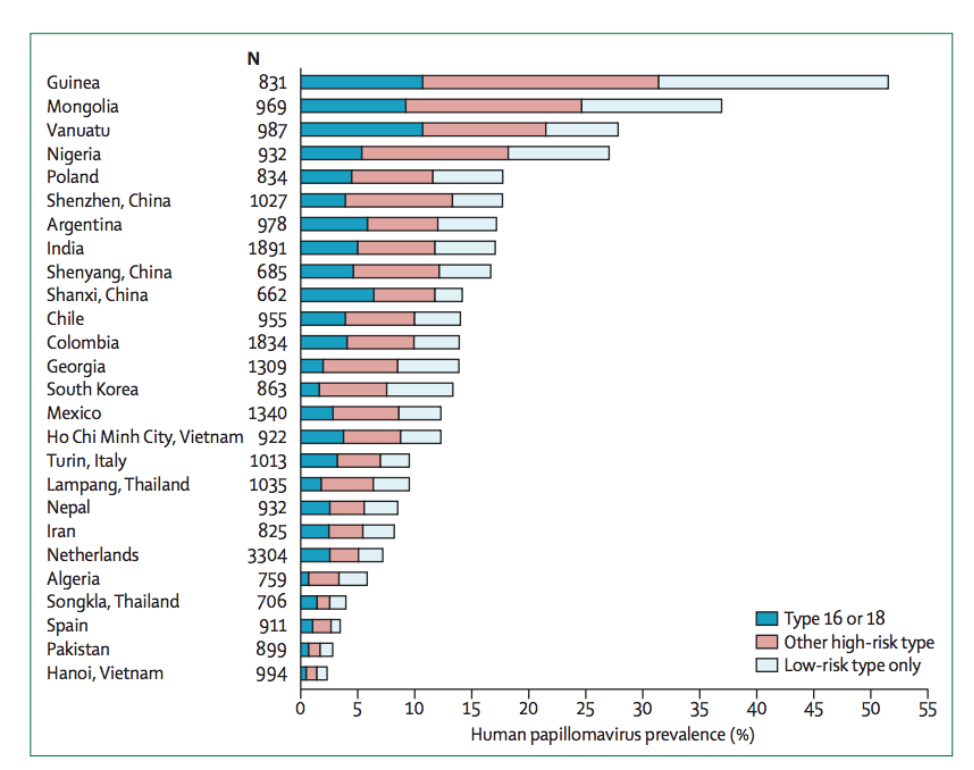
\includegraphics[scale=0.7]{IMG/prevalence.png}
	\caption{Age\-adjusted prevalence of cervical human papillomavirus DNA in sexually active women aged 15\-69 years. Data are from IARC Prevalence Surveys, 1990\-2012.4}
	\label{zurHausen}
\end{figure} 
%Foto de prevalencia


%Literatura
Most people who become infected with HPV do not know they have it. Usually, the body's immune system gets rid of the HPV infection naturally within two years. This is true of both HR and LR types. By age 50, at least 4 out of every 5 women will have been infected with HPV at one point in their lives. HPV is also very common in men, and often has no symptoms.

When the body's immune system can't get rid of a HR HPV infection, it can linger over time and turn normal cells into abnormal cells and then cancer. About 10\% of women with HR HPV on their cervix will develop long-lasting HPV infections that put them at risk for cervical cancer. Similarly, when HR HPV lingers and infects the cells of the vulva, vagina, penis, anus, or the oropharynx (back of the throat, including the base of the tongue and tonsils), it can cause cell changes called precancers. These may eventually develop into cancer if they're not found and removed in time. These cancers are much less common than cervical cancer. Much less is known about how many people with HPV will develop cancer in these areas.

%Empiezon con las vacunas
Since the release of the first vaccines in 2006, nowadays there are three available: a quadrivalent (including HPV genotypes 16, 18, 6 and 11) and a bivalent vaccine (including genotypes 16 and 18) and a nonavalent (including genotypes 6, 11, 16, 18, 31, 33, 45, 52 and 58). All vaccines are efficacious to protect against precancerous lesions in the cervix, vulva or vagina; in addition, the quadrivalent and nonavalent prevent precancerous anal lesions, anal cancer and anogenital warts.

\begin{figure}[ht]
	\centering
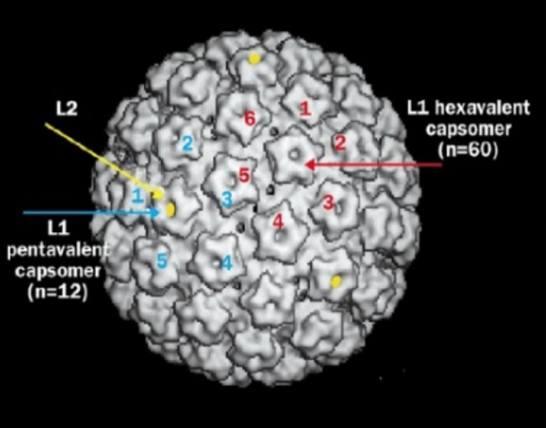
\includegraphics[scale=0.7]{IMG/cryo.png}
\caption{Structure of a HPV virus-like particle. A three-dimensional reconstruction of a cryolectron micrograph (cryo-EM) of a virus-like particle (VLP) is shown. The VLP is composed of 60 hexavalent capsomers and 12 pentavalent capsomers, all consisting of pentamers of L1 protein. The L2 protein is not visible by cryo-EM but is tought to be associated with the pentavalent capsomers, and have been colored in yellow.}
\label{cryo}
\end{figure}  

According to the Advisory Committee on Immunization Practices (ACIP) from the Centers for Disease Control (CDC) and Prevention, new recommendations are given for use of a 2-dose schedule for girls and boys who initiate the vaccination series at ages 9 through 14 years. Three doses remain recommended for persons who initiate the vaccination series at ages 15 through 26 years and for immunocompromised persons.

In Spain HPV vaccine is given to adolescent girls as part of the national immunization programme, and is recommended at different age groups in different Autonomous Communities. Numerous cost-effectiveness studies of HPV-vaccination have been published in other countries. However, few studies include the prophylactic effect of all HPV-associated diseases, or the impact of vaccinating men.

There are countries that recommend also vaccinating boys in order to decrease the burden of disease in them. Some models have shown that the female vaccination program has some herd immunity and the impact of implementing the vaccination in males may not be cost effective, however not vaccinating males leaves them at risk of cancers, especially the groups that do not benefit of the herd immunity, as the males that have sex with males.
Besides, there is no economic analysis of the nonavalent program in Spain, and it is important from the decision making perspective.

Even with the high prevalence of sexually transmitted diseases there are few studies devoted to ascertain the structure of sexual networks and its role in disease transmission. Most studies are restricted to small communities such as the Jefferson High Schools project (P. S. Bearman et al., Chains of Affection: The Structure of Adolescent Romantic and Sexual Networks, American Journal of Sociology, 110(1) (2004) 44-91) or that of Likoma Island (S. Helleringer and H. P. Kohler, Sexual network structure and the spread of HIV in Africa: evidence from Likoma Island, Malawi, AIDS 21 (2007) 2323-2332).

Random network mathematical models may simulate the interactions and propagations of all these viruses through sexual contacts among a population of more than one million people (including heterosexual and homosexual populations). As this model is based upon a network instead of traditional continuous model approaches (E. H. Elbasha et al., Model for assessing human papillomavirus vaccination strategies,  Emerging. Inf. Dis.  2007; 13:28-41) we will be able to determine with higher accuracy the effect of vaccination in a short and large periods of time.

